\documentclass{article}
 

\usepackage{amsmath}
\usepackage{amssymb}
\usepackage{graphicx}
\usepackage{verbatim}
\usepackage{enumerate}
\usepackage{hyperref}
\usepackage{subcaption}
\usepackage{ifoddpage}

\newcommand{\beq}{\begin{equation}}
\newcommand{\eeq}{\end{equation}}

\begin{document}
\title{Project 5. FYS3150}
\author{Candidate nr. 2 collaboration with cand. nr. 20}
\maketitle
\newpage

%----------------------------INTRO-----------------------------------
%%%%%%%%%%%%%%%%%%%%%%%%%%%%%%%%%%%%%%%%%%%%%%%%%%%%%%%%%%%%%%%%%%%%%
%--------------------------------------------------------------------
\section{Introduction: N-body simulation of an open galactic cluster}
\begin{figure}[h!]
  \centering
  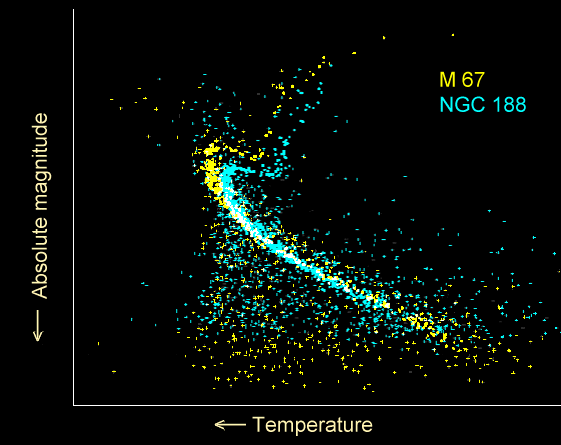
\includegraphics[scale=0.5]{fig.png}
  \caption{fig1: Herzsprung-Russel diagrams for the two open clusters M67 and NGC188. Most of the NGC188's stars are on the main sequence, but some if its heaviest stars are starting to leave the main sequence indicating its age. We also see the younger cluster M67 following closely after as comparison.}
\end{figure}

The goal of this project will be developing a code that will perform simulations of an open cluster using Newtonian gravity. The project is inspired by the article \textit{Cold uniform spherical collapse revisited} \cite{art}
Before we embark on the journey, we shall first of all, see the two methods we are going to use and the stability of these two for the whole system consisting of N bodies. We start with a two body problem and then go on to N-body problem. Along the way we shall see which of the methods is better than the other and then choose the one best fitted for our purpose to carry on further calculations. 

We will proceed making an animation of the N-body in three dimension and calculating the energies of the particles, will the energy be conserved? And how long time will it take for the system to reach equilibrium? We will implement a new model for the system after a few calculations which takes into account the numerical instabilities that occur when two bodies are close to each other and then test the physical properties for this new model. 

After presenting the methods, results we will wrap up with a conclusion and discussion. 

\subsection{Leap-Frog algorithm}
We start by noting Newton's second law:
$$m\frac{d^2x}{dt^2} = F(x,t)$$ 
Further we have the relations $x^{(2)}(t) = a(x, t)$ and $x^{(1)} = v(x,t)$ in other words the second derivative of the position is equal to the acceleration and the first derivative equal to the velocity.
Using the two relations we can write our equation:
$$\frac{dx}{dt} = v(x,t) \hspace{1cm} \frac{dv}{dt} = \frac{F(x,t)}{m} = a(x,t)$$ 
Performing a Taylor expansion:
$$x(t+h) = x(t) + hx^{(1)}(t) + \frac{h^2}{2}x^{(2)}(t) + O(h^3)$$
We can now use our relation from above and add the corresponding $x(t-h)$ to obtain:
$$x(t_h \pm h) = x_{i\pm1} \hspace{2cm} x_i = x(t_i)$$
$$x_{i+1} = 2x_i - x_{x-1} + h^2x_i^{(2)} + O(h^4)$$
where we have the truncation error as $O(h^4)$ as a result of adding the $x(t - h)$ term. 
In our calculation we would know the velocity, if however we wish  to know the velocity we could find it by:
$$x_i^{(1)} = \frac{x_{i+1} - x_{i-1}}{2h} + O(h^2)$$
With truncation error as $Oh^2$. 
Now if we just rewrite our Taylor equation from the Verlet formula we can get the Leap-Frog:
$$x(t+h) = x(t) + h\left(x^{(1)}(t) + \frac{h}{2}x^{(2)}(t)\right)$$
We have:
$$x(t+h/2) =\left(x^{(1)}(t) + \frac{h}{2}x^{(2)}(t)\right)$$
And obtain:
$$x(t+h) = x(t) + hx^{(1)}(t + h/2)$$
combining it with our equation:
$$x^{(1)}(t + h/2) = x^{(1)}(t - h/2) + hx^{(2)}(t)$$
Now we see that the velocity and the position are computed at different time steps, so in order to get it at time $t$ we can use:
$$x^{(1)}(t) = \left(x^{(1)}(t \mp h/2) \pm \frac{h}{2}x^{(2)}(t)\right)$$
To sum up, the velocity and the position are calculated at different time steps and the final algorithm becomes:
\begin{align*}
x(t+h/2) =& x^{(1)}(t) + \frac{h}{2}x^{(2)}(t)\\
x(t+h) =& x(t) + hx^{(1)}(t + h/2)\\
x^{(1)}(t+h) =& x(t+h/2)+ \frac{h}{2}x^{(2)}(t)
\end{align*}


\subsection{Runge-Kutta 4 (RK4)}
Here we will simply show the basic idea and concept of our second method of choice. The general idea behind RK4 is finding solutions for ODE's, consider having an ODE on the form:
$$\frac{dy}{dt} = f(t,y) $$ 
such that:
$$y(t) = \int f(t,y)$$
$$y_{i+1} = y_i + \int_{t_i}^{t_{i+1}} f(t,y)$$
Hence the basic philosophy is that it gives us an intermediate step in the computation of $y_{i+1}$. For the full derivation see \cite[p.~251]{compf}
Here we will simply state the algorithm. first we compute
$$K_1 = hf(t_i,y_i)$$
Which is exactly the Euler method at this stage, taking a step further and using Euler's method to compute a slope at the midpoint $y_{i+1/2}$. So far all the same as the second order Runge-Kutta.
$$K_2 = hf(t_i+h/2, y_i + K_1/2)$$
Then we use the new slope we found to further improve the slope at $y_{i+1/2}$ by
$$K_3 = hf(t_i + h/2, y_i + K_2/2)$$
With the latter slope we can then compute $y_{i+1}$ with
$$K_4 = hf(t_i + h, y_i + K_3)$$
With which we finally get:
$$y_{i+1} = y_i + \frac{1}{6}(K_1+2(K_2+K_3) + K_4)$$

%-----------------------END OF INTRO-----------------------------
%%%%%%%%%%%%%%%%%%%%%%%%%%%%%%%%%%%%%%%%%%%%%%%%%%%%%%%%%%%%%%%%%
%----------------------------------------------------------------



%--------------------METHODS------------------------------------
%%%%%%%%%%%%%%%%%%%%%%%%%%%%%%%%%%%%%%%%%%%%%%%%%%%%%%%%%%%%%%%%%
%----------------------------------------------------------------
\section{Methods}
In this section we will implement the two methods and carry out calculations to compare the two. As for the implementation it is mostly straight forward as we follow the schemes closely as described above.
\subsection{Leap-Frog}
\begin{verbatim}
1   mat SolarSystem::LF(mat SV){
2       double dt = 0.001;
3    
4       dSVdt = derivative(SV); 
5       mat V1 = SV.submat(0,3,N-1,5) + dt/2.0*(dSVdt.submat(0,3,N-1,5));
6       
7       SV.submat(0,0,N-1,2) += dt*SV.submat(0,3,N-1,5);
8       dSVdt = derivative(SV);
9       SV.submat(0,3,N-1,5) = V1 + dt/2.0*(dSVdt.submat(0,3,N-1,5));
10
11      return SV;
    }
\end{verbatim}
The implementation is as follows, line \texttt{2} is the step size corresponding to $h$ in the Leap-Frog algorithm, then we have a six dimensional matrix with three space coordinates and three velocity coordinates that we obtain using the function \texttt{derivate} (see the attachment for the complete code). Line \texttt{5} corresponds to the half step velocity calculation in the Leap-Frog scheme $x^{(1)}(t+h/2)$. Here we take the sub-matrix of our six dimensional matrix corresponding to the three velocity coordinates. and then times the half step length times the derivative matrix, which contains three velocity coordinates and three acceleration. In line \texttt{7} we find the position at time step $h$, where we again this take the sub-matrix, this time the space coordinates and then times the step length times the velocity. Then we update the derivative at line \texttt{8} by running it through the function \texttt{derivative} before finally calculating the velocity (line \texttt{9}), this time at time step $h$. To get the values we run the function in a loop of a desired time length.
\newpage
\subsection{RK4}

\begin{verbatim}

 mat SolarSystem::RK4(mat SV){
1  double dt = 0.001;
2  mat K1,K2,K3,K4 = zeros(N,6);
3  K1 = derivative(SV);
4  K2 = derivative(SV + (K1/2)*dt);
5  K3 = derivative(SV + (K2/2)*dt);
6  K4 = derivative(SV + K3*dt);
7  SV += (1/6.0)*dt*(K1 + 2*(K2 + K3) + K4);
8  
9  return SV;
 }
\end{verbatim}
Here as well as before we have a time step \texttt{dt} corresponding to our $h$ in the scheme lines $3$ - $7$ follow exactly the method as we described it. In line $3$ we find the first slope which corresponded to the Euler method at point $t_i$ and go on from there in line \texttt{4} and \texttt{5} we find the second order RK by taking the previous slope to predict $y_{i+1/2}$ and then at the next line using it to further improve the slope at $y_{i+1/2}$. Lastly we add the terms together to find $y_{i+1}$ which in this case corresponds to our updated values of the position and velocity matrix. 

\subsection{Comparison}
We shall start comparing the two methods for different values of $N$ and see the outcome, here we list a few of them.\\ 

\begin{tabular}{l|*{6}{c}r}
dt                & t         & Leap-Frog   & Runge-Kutta &\\
\hline
0.1               & 1000      &             &\\
0.01              & 100       & 3           &\\
0.001             & 10        & 2           &\\
0.0001            & 1         & 2           &\\
\end{tabular}
%-----------------END OF METHODS-----------------------
%%%%%%%%%%%%%%%%%%%%%%%%%%%%%%%%%%%%%%%%%%%%%%%%%%%%%%%
%-----------------------------------------------------

%------------------RESULTS------------------------------
%%%%%%%%%%%%%%%%%%%%%%%%%%%%%%%%%%%%%%%%%%%%%%%%%%%%%%%%
%-------------------------------------------------------
\newpage
\section{Results}
We now want to extend our code a bit further and generalize for N-body problem.
With the given conditions of unit length in light years and mass in solar mass, we are wondering
how long we could realistically expect the cluster to collapse. To achieve this
we run a simple code to simulate a 10 solar mass object. We set initial condition x0=20ly
v0=0, being pulled towards another object of 100 solar mass, it returned 25 million years as
the time of contact. From this simple model we can see that our model in which the
particles are uniformly scattered will result in a much slower progress, but our time
should still be in the order of 10million-100million years.

The current model isn't without it's weakness, we can't expect results that 
would otherwise be observed in nature such as singulary after a collapse of a cluster. 
From the initial conditions set, both N approaching infinity and density like that of continuous fluid,
it's clear that we won't get the same outcome. Our particles pass through eachother and do not have 
force that bonds them in a way fluids would. We have few but large objects that rarely interact except 
for when they 'collide' and gain high velocities. There isn't a way to lump together mass at the center
if it can escape through the large space  between objects and it has not bonding force with nearby objects.

That said we can't have high expectation of such a simple model. We will however run simulations on this model and see
if there are any worthwhile results.

Having completed the implementation of the model we move on to simulating a system of 200 particles for t'= 3 crunch time.
From the movie it's easy to see the different stages of the simulation, we observe that the crunch happens at t' = 1 by
the number of particles that have gathered at the center. As we watch we see the center of the cluster expanding at 
very fast rate, by the time t'=1.5 crunch time the explosive expansion has been slowed down and we conclude that the
bound particles are in equilibrium.
\begin{figure}[h!]
  \centering
  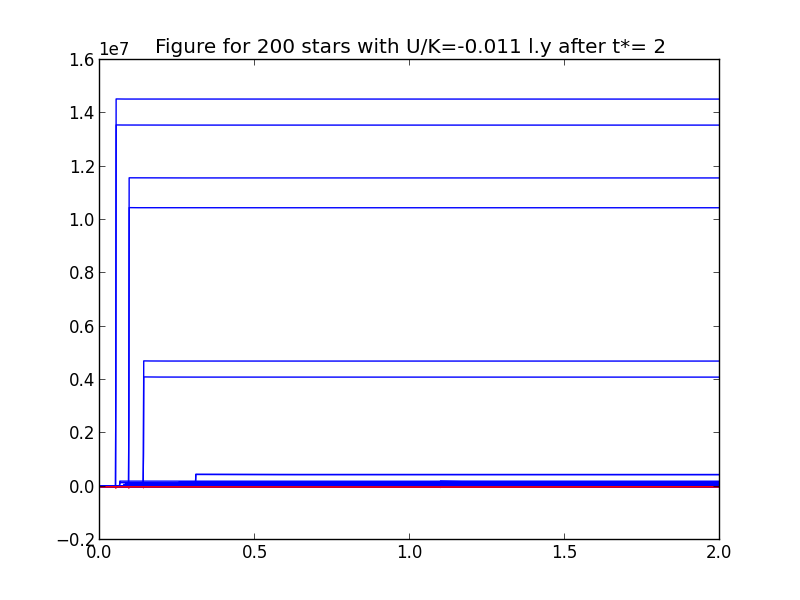
\includegraphics[scale=0.5]{d1-200.png}
  \caption{fig2:A look at the energies for 200 particle system.}
\end{figure}
We study a system of 10,50,100, 150 and 200 particles. We want to see
how the size of the cluster relates to the varius quantities we measure.
We set a condition for ejection which is all particles that venture outside
of a sphere with radius 45 ly. We then count the particles within our sphere
and see a near constant ratio of bound particles  versus ejected particles. 
\begin{verbatim}
|Total: Ejected|
|200  :      49|
|150  :      40|
|100  :      24|
|50   :      16|
|10   :       4|
\end{verbatim}
We start with 40\% ejection rate for 10 particles, then 32\%, then 24\%, then 26.6\% and
lastly 24.5\%.
With this we also measure the energy of the ejected particles versus the energy of the
total system and observe:

\begin{verbatim}
100.33% of the systems total energy for 200 particles
100.9% of the systems total energy for 150 particles
100.02% of the systems total energy for 100 particles
119.28% of the systems total energy for 50 particles
100.59% of the systems total energy for 10 particles
\end{verbatim}

Only the energies of 50 particle system stands out, with lower system energy than otherwise expected.
However we observe the larger trend where we have a very large part of the systems energy in the 
ejected particles.

On the conservation of the energy in the system:
The energy is not conserved, we start out with a negative total energy 
due to the kinetic energy being zero. We end up with huge kinetic energy
for the system once the particles start interacting and some of them are
ejected. We plot the kinetic and potential energy and see that for
some particles their kinetic energy is 100s of times larger than their
potential energy. Due to the kinetic energy being proportional to
$v^2$ we can easily see which particles are ejected by their kinetic energy.
But this is not all, we also observe that for the ejected particles, their
kinetic energy remains near constant, which tells us that it has escaped
far enough to not be pulled in by the gravitational force which is proportional
to $1/r^2$. Which if we ignore the force between the ejected particles 
is the radius to the center mass of the bound particles.


\begin{figure}
\centering
\begin{subfigure}{.7\textwidth}
  \centering
  \hspace{-6cm}
  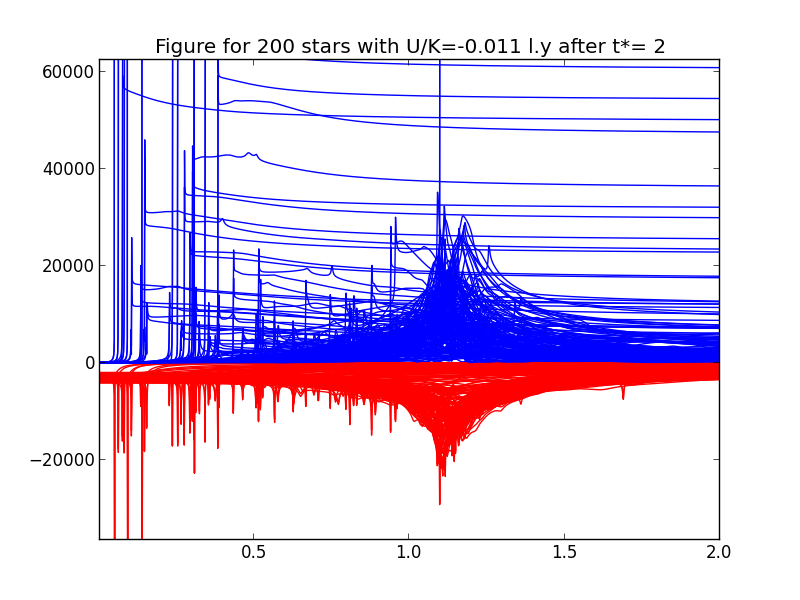
\includegraphics[scale=0.5]{d2-200.png}
  \caption{fig3:A look at the energies for 200 particle system zoomed in.}
  \hspace{-6cm}
  \label{fig:sub1}
\end{subfigure}%
\begin{subfigure}{.7\textwidth}
  \hspace{-5cm}
  \centering
  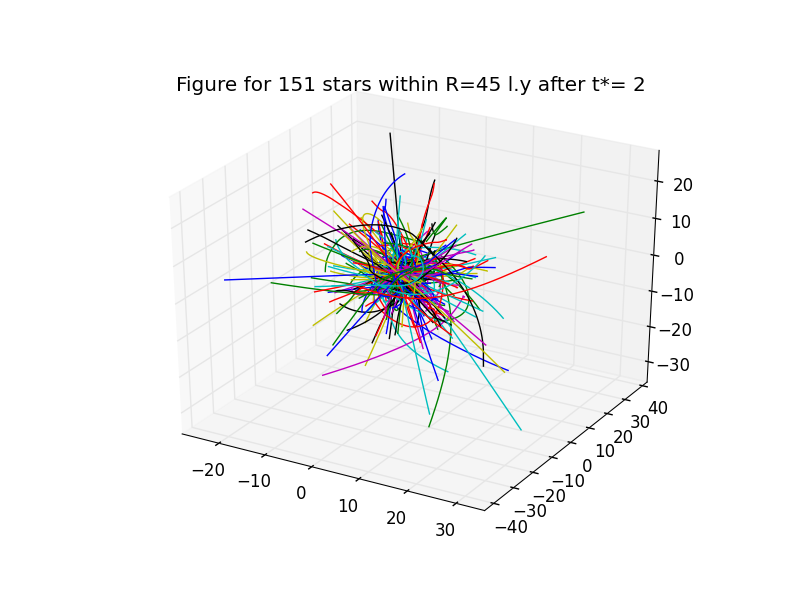
\includegraphics[scale=0.4]{d3-200.png}
  \caption{fig4:A look at 3D trajectory for 200 particle system.}
  \label{fig:sub2}
\end{subfigure}
\label{fig:test}

\end{figure}

%\newpage
%\begin{figure}
%  \centering
 % \begin{subfigure}[b]{0.4\textwidth}
  %  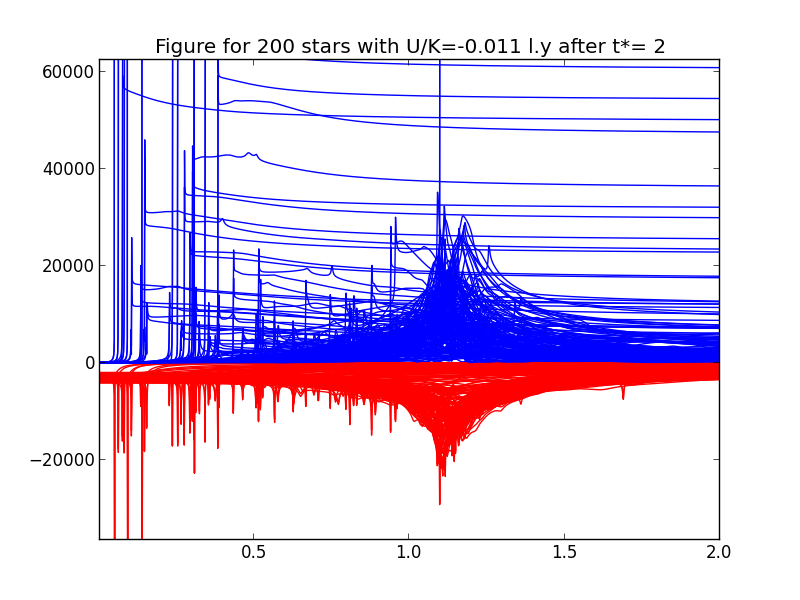
\includegraphics[scale=0.4]{d2-200.png}
   % \caption{fig3:A look at the energies for 200 particle system zoomed in.}
  %\end{subfigure}


%  \begin{subfigure}[b]{0.4\textwidth}
 % 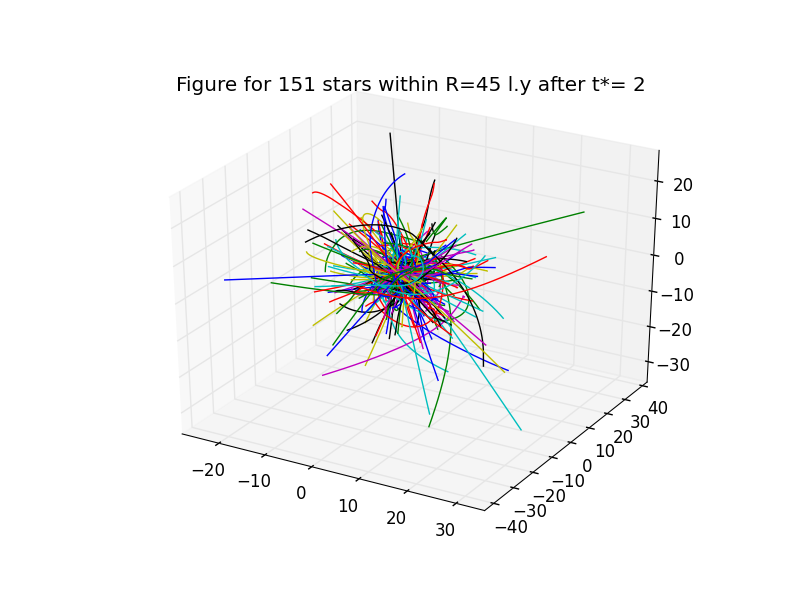
\includegraphics[scale=0.4]{d3-200.png}
 % \caption{fig4:A look at 3D trajectory for 200 particle system.}
 % \end{subfigure}
%\end{figure}

We study the 200 particle simulation in fig3, here we observe that there are sharp increase
in kinetic energy between $t'=0.5$ and 1.5. However most of these are exponentially 
decreasing after their maxima. This, we hypothisize, is due to the density of particles
in the area of the sphere this takes place. Our hypothesis is further strengthened by
the decreasing likelihood of their appearence as time moves towards crunch time and beyond.
We understand this is due to the large force that now acts on these over smaller distance
it's more difficult to escape than when the particles were scattered uniformly in the sphere.
As we reach equilibrium we see that these sharp increases have disappeared completely, and we
conclude that it must be because of the mass concentrated in the center of the cluster and the 
total force that acts on particles so close to the center of the cluster.
We included a 3D figure of the bound particles above.
%%----------------------------
\begin{figure}
\centering
\begin{subfigure}{.65\textwidth}
  \centering
  \hspace{-6cm}
  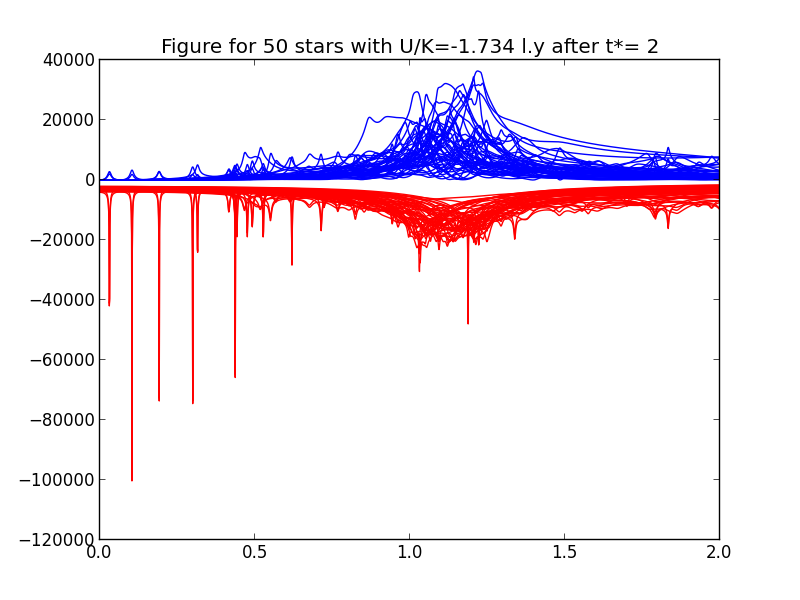
\includegraphics[scale=0.45]{e1-50.png}
  \caption{fig5:A look at the energies for 50 particle system with $\epsilon$.}
  \hspace{-6cm}
  \label{fig:sub1}
\end{subfigure}%
\begin{subfigure}{.65\textwidth}
  \hspace{-5cm}
  \centering
  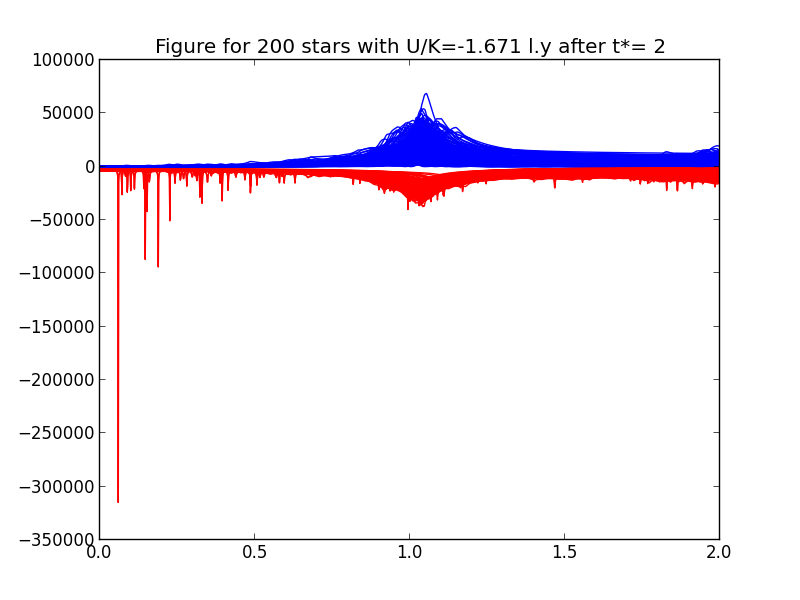
\includegraphics[scale=0.45]{e1-200.png}
  \caption{fig6:A look at energies for 200 particle system also with $\epsilon$.}
  \label{fig:sub2}
\end{subfigure}
\label{fig:test}

\end{figure}


%\newpage
%\begin{figure}[h!]
%  \centering
%  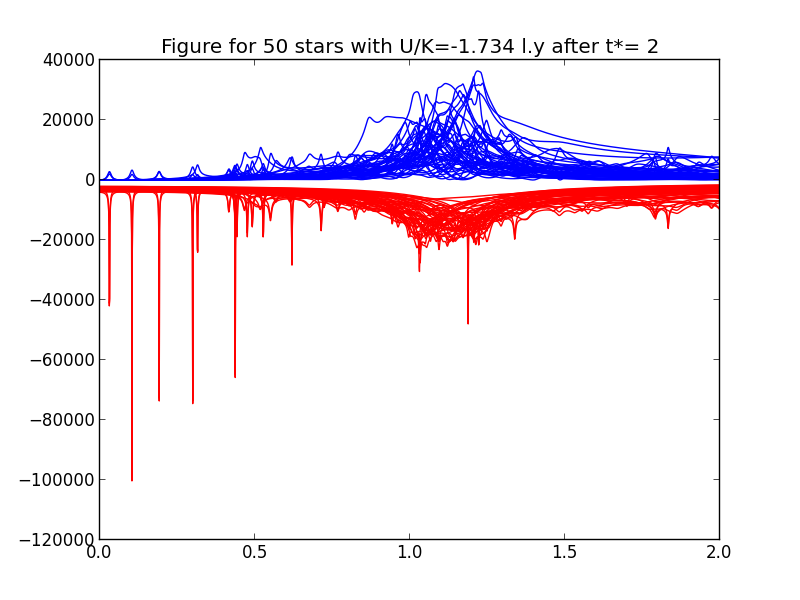
\includegraphics[scale=0.4]{e1-50.png}
%  \caption{fig5:A look at the energies for 50 particle system with $\epsilon$.}
%  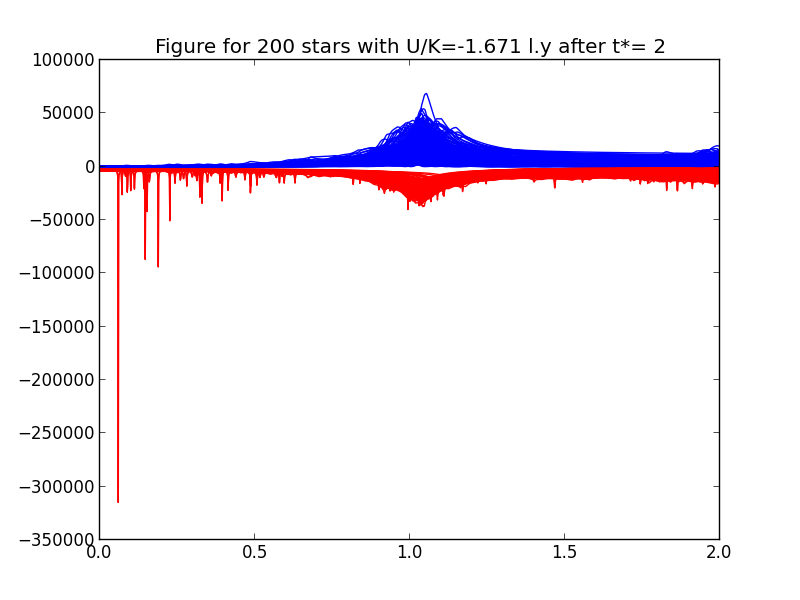
\includegraphics[scale=0.4]{e1-200.png}
%  \caption{fig6:A look at energies for 200 particle system also with $\epsilon$.}
%\end{figure}

So we have done computation and found our model lacking, there are physical
phenomenas that aren't being observed at all, and our model lacks functionality.
We want to change our model according to the project file and see if the results
are any better.

We add a term to our equation for the force so we avoid particles
almost being on top of eachother and thus creating the problem of 
particles escaping with huge velocities. It also makes particles lump together
as they can't shoot past eachother when they are very close.

Adding this term epsilon to the denominator has done wonders for our algorithm.
We no longer observe particles that have escaped with such velocities
that the potential and kinetic energies of bound particles look
like constants (fig2). We observe a sharp decrease in the number of particles that
have been ejected, at 200 it has gone from 24.5\% to 4\%. The biggest change being
50 particle system where we previously had 32\% we now have 0\% ejected particles.

We look at the energies and following the trend we described above, it's only
expected that the energies of the ejected particles also decrease sharply.

We measure the energy of the ejected particles versus the energy of the
total system and observe:
\begin{verbatim}
6.7% of the systems total energy for 200 particles 
7.22% of the systems total energy for 150 particles
3.51% of the systems total energy for 100 particles
0% of the systems total energy for 50 particles
\end{verbatim}
\newpage
\begin{figure}
\centering
\begin{subfigure}{.65\textwidth}
  \centering
  \hspace{-6cm}
  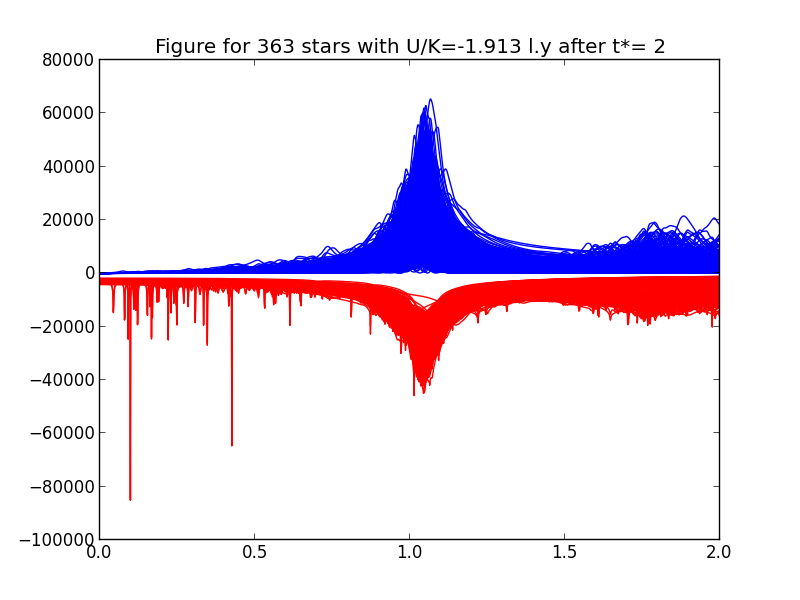
\includegraphics[scale=0.45]{f1-400.png}
  \caption{fig7: A look at the energies for 400 particle system.}
  \hspace{-6cm}
  \label{fig:sub1}
\end{subfigure}%
\begin{subfigure}{.65\textwidth}
  \hspace{-5cm}
  \centering
  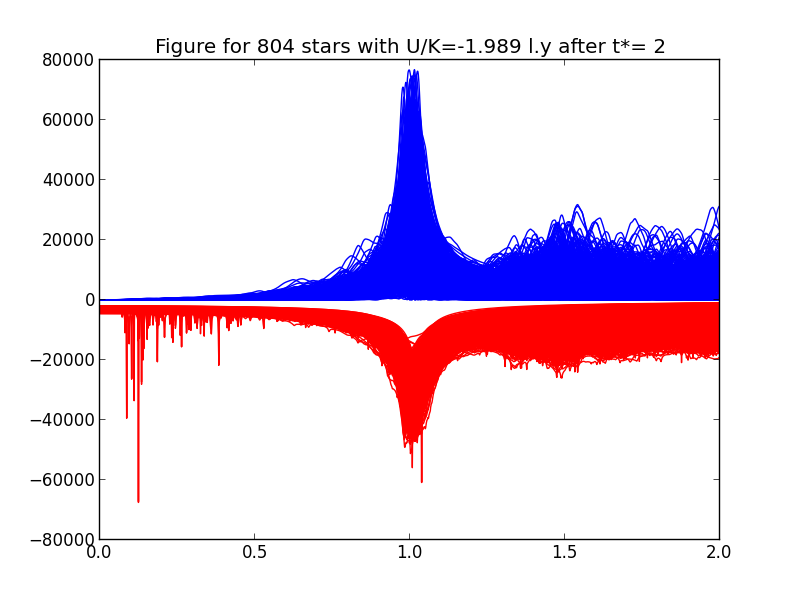
\includegraphics[scale=0.45]{f1-1000.png}
  \caption{fig8:A look at energies for 1000 particle system.}
  \label{fig:sub2}
\end{subfigure}
\label{fig:test}

\end{figure}
%\begin{figure}[h!]
%  \centering
%  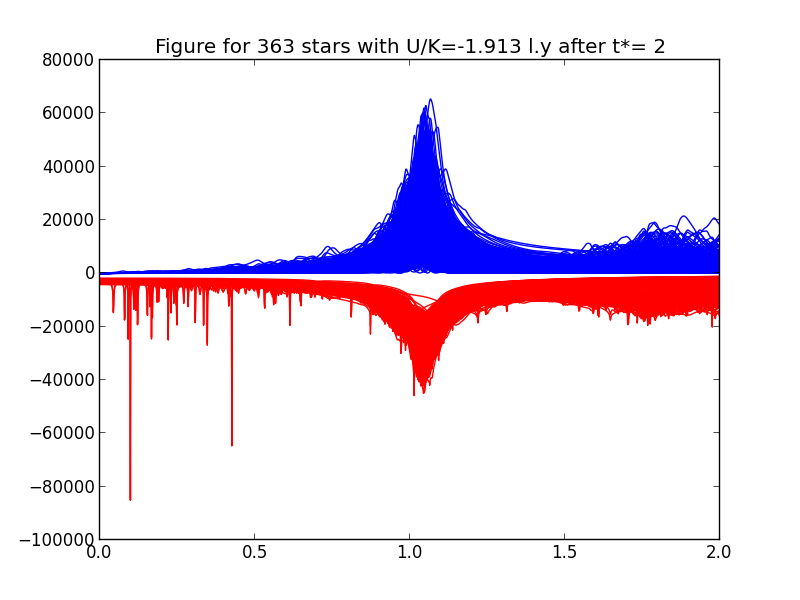
\includegraphics[scale=0.4]{f1-400.png}
%  \caption{fig7: A look at the energies for 400 particle system.}
%  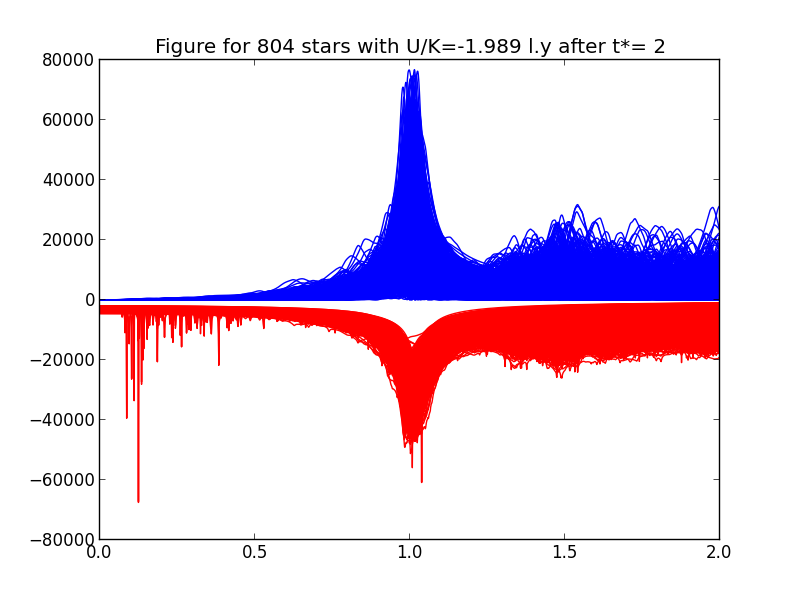
\includegraphics[scale=0.4]{f1-1000.png}
%  \caption{fig8:A look at energies for 1000 particle system.}
%\end{figure}

Next for a measurement of kinetic energy and potential energy and
the Virial theorem. The Virial Th. states that $2<K>=-<U>$ which
tells us that the average potential energy is twice the negative of
the kinetic energy of a system that obeys this law.
To start we want to run our simulations again, this time we will
measure the ratios and how the number of particles in the system
changes it.

We chose a sphere of radius R=2R0 for a time t'= 2.
We started with the same numbers of particles as before, we see at
50 particles we have -1.73 ratio, which is not all that bad for such
a simple simulation, as we increase the number of particles we notice
that the ratio increases and moves towards 2, but we also notice that
the ratio of bound particles decreases. From our previous algorithm
we had for increasing N a ejection rate decreasing towards 25\%. For
this new algorithm, we started with 0\% and at 1000 particles we have 19.6\%.
We cannot make assumptions beyond the fact that the system will look to settle
at a rate as N increases. With this in mind, we observe the trend in the ratio
of potential and kinetic energy. A low of -1.73 for 50 particles to a high of
-1.988 for a system of 1000 particles. From this we can say that as N increases
it fulfills the condition of the Virial Theorem.
\begin{verbatim}
|N   |Bound|ratio U/K|
|1000|  804|-1.988   |
|400 |  363|-1.91    |
|200 |  183|-1.90    |
|150 |  143|-1.81    |
|100 |   94|-1.80    |
|50  |   50|-1.73    |
\end{verbatim}


\newpage
\begin{figure}[h!]
  \centering
  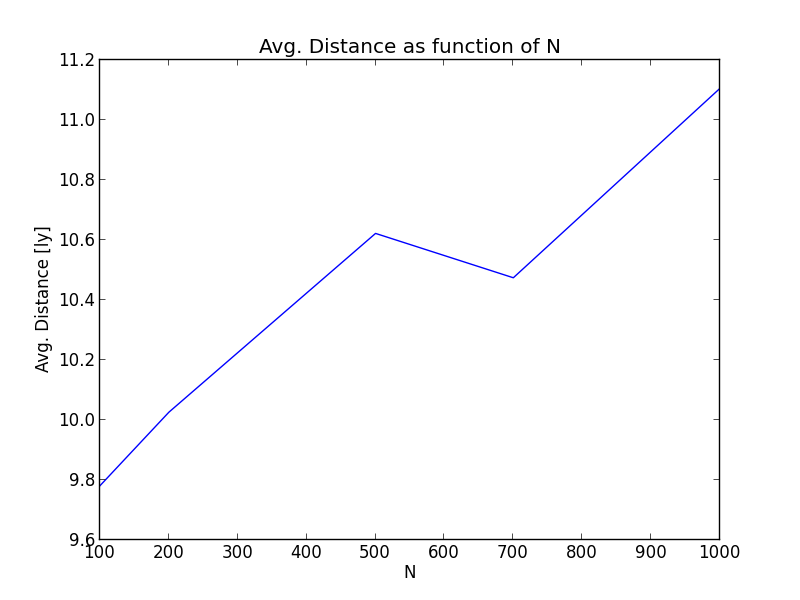
\includegraphics[scale=0.4]{g3.png}
  \caption{fig9: A look at average distance as function of N.}
\end{figure}
We will create a sphere (S0) of radius r0 and divide the particles (p0) in the sphere by the volume.
We will then create another sphere (S1) of radius r1 and substract particles (p1) in S1 by particles(p0) in S0.
We will then divide that by the volume of S1 substracted from S0. Such as:(p1-p0)/(s1-s0) to find the particle
density of volume between $r_0<r<r_1$ And so on.
\begin{verbatim} 4*pi*((i+1)*dr)**3/3 - 4*pi*(i*dr)**3/3 \end{verbatim}
We calculate the Avg. distance, standard div. and average distance as function of N.
Average distance varies little, the standard div. varries little for 500 particles and 1000.
However the average distance as function of N shows interesting feature. It is increasing for all 
except one point, and the increase as function of N is 0.15 for ever 100 N.
\begin{verbatim} 
Average Distance: 10.026 standard div.: 6.88257 for N=200
Average Distance: 10.6219 standard div.: 7.93572 for N=500
Average Distance: 10.4741 standard div.: 8.46936 for N=700
Average Distance: 11.1056 standard div.: 9.62076 for N=1000
\end{verbatim} 

\begin{figure}
\centering
\begin{subfigure}{.65\textwidth}
  \centering
  \hspace{-6cm}
  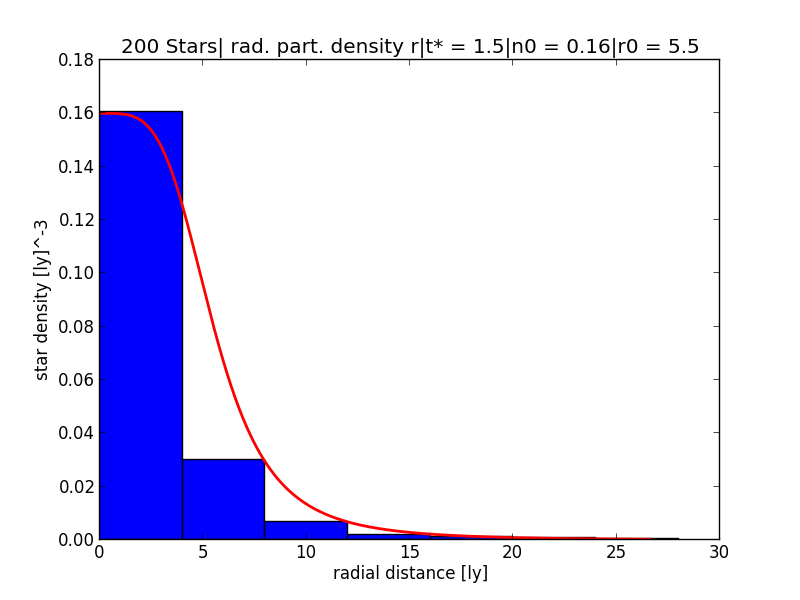
\includegraphics[scale=0.45]{g1-200.png}
  \caption{fig10: Radial density of 200 particle system.}
  \hspace{-6cm}
  \label{fig:sub1}
\end{subfigure}%
\begin{subfigure}{.65\textwidth}
  \hspace{-5cm}
  \centering
  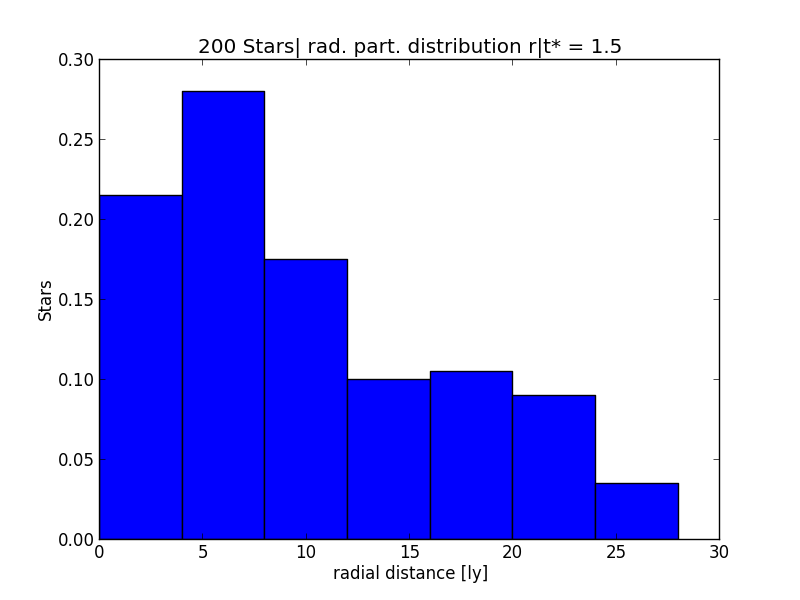
\includegraphics[scale=0.45]{g2-200.png}
  \caption{fig11: Radial distribution of particle 200 particle system.}
  \label{fig:sub2}
\end{subfigure}
\label{fig:test}
\end{figure}


\begin{figure}
\centering
\begin{subfigure}{.65\textwidth}
  \centering
  \hspace{-6cm}
  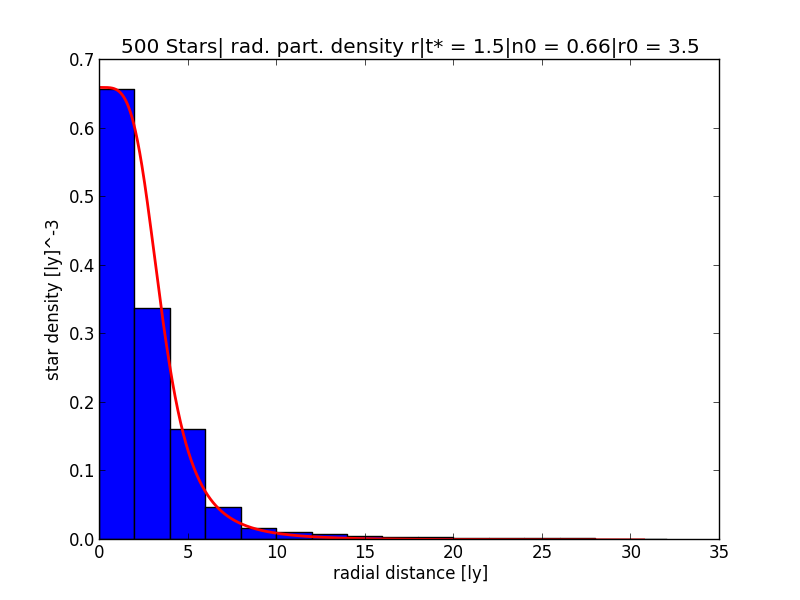
\includegraphics[scale=0.45]{g1-500.png}
  \caption{fig12: Radial density of 500 particle system.}
  \hspace{-6cm}
  \label{fig:sub1}
\end{subfigure}%
\begin{subfigure}{.65\textwidth}
  \hspace{-5cm}
  \centering
  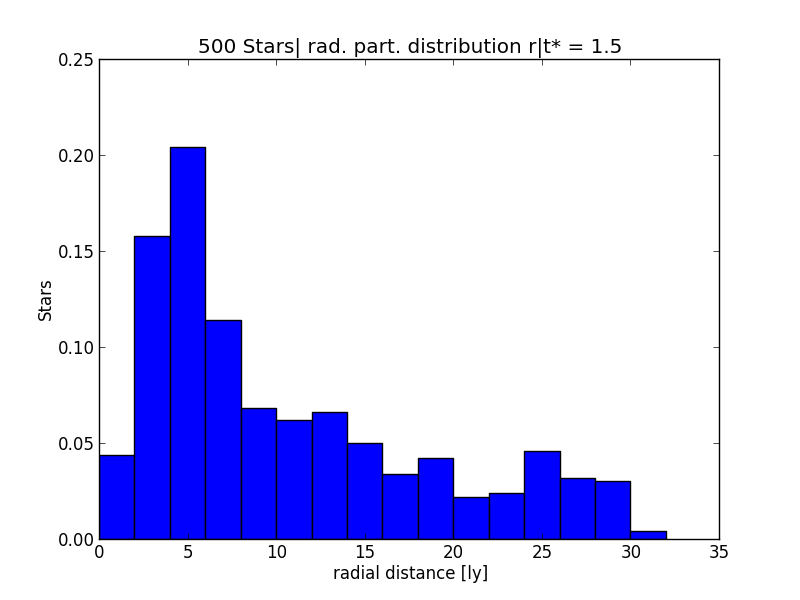
\includegraphics[scale=0.45]{g2-500.png}
  \caption{fig13: Radial distribution of particle 500 particle system.}
  \label{fig:sub2}
\end{subfigure}
\label{fig:test}
\end{figure}

\begin{figure}[h]
  %\setcapwidth{0.6\textwidth}
  \checkoddpage
  \edef\side{\ifoddpage l\else r\fi}%
  \makebox[\textwidth][\side]{%
    \begin{minipage}[t]{0.59\textwidth}
      \centering
      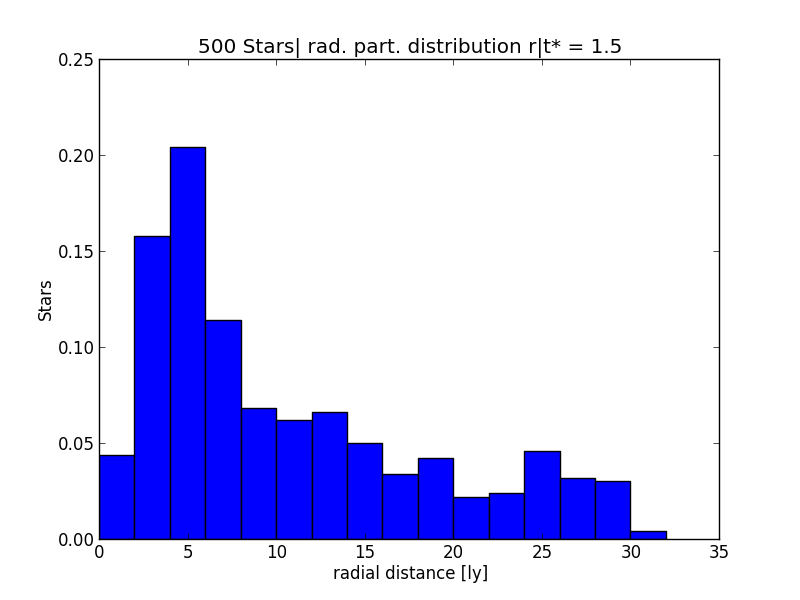
\includegraphics[width=\textwidth]{g2-500.png}
      \caption{Caption 1}
    \end{minipage}%
    \hfill
    \begin{minipage}[t]{0.59\textwidth}
      \centering
      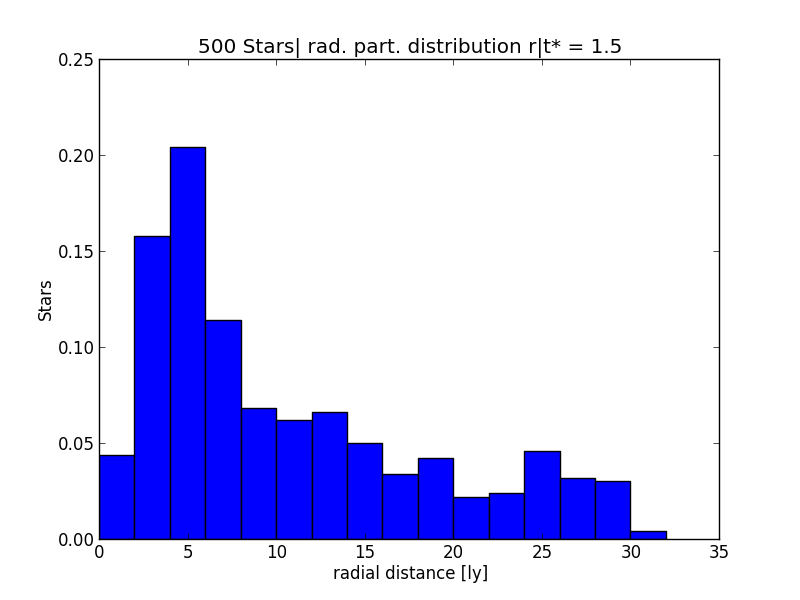
\includegraphics[width=\textwidth]{g2-500.png}
      \caption{Caption 2}
      \label{fig:free-lunch}
    \end{minipage}%
  }%
\end{figure}

%----------------------END OF RESULTS------------------
%%%%%%%%%%%%%%%%%%%%%%%%%%%%%%%%%%%%%%%%%%%%%%%%%%%%%%%
%------------------------------------------------------


%------------------CONCLUSION---------------------------
%%%%%%%%%%%%%%%%%%%%%%%%%%%%%%%%%%%%%%%%%%%%%%%%%%%%%%%%
%-------------------------------------------------------
\newpage
\section{Conclusion}



%-------------------END OF CONCLUSION------------------
%%%%%%%%%%%%%%%%%%%%%%%%%%%%%%%%%%%%%%%%%%%%%%%%%%%%%%%
%------------------------------------------------------

%-------------------REFERENCES-------------------------
%%%%%%%%%%%%%%%%%%%%%%%%%%%%%%%%%%%%%%%%%%%%%%%%%%%%%%%
%------------------------------------------------------
\newpage
\begin{thebibliography}{9}

\bibitem{compf}
  M.H. Jensen
  \emph{Computational Physics}.
  University of Oslo.
  2013

\bibitem{art}
  M.Joyce, B.Marcos and F.Sylos Labini
  \emph{Cold uniform spherical collapse revisited}.
  \url{http://arxiv.org/abs/1011.0614}
  2011

\bibitem{cite1}
\emph{animation example code: simple\_3danim.py}
\url{http://matplotlib.org/1.3.0/examples/animation/simple_3danim.html}

\end{thebibliography}

%------------------END OF PROJECT----------------------------
%%%%%%%%%%%%%%%%%%%%%%%%%%%%%%%%%%%%%%%%%%%%%%%%%%%%%%%%%%%%%
%------------------------------------------------------------

\end{document}
